\documentclass[a4paper,10pt]{article}
\usepackage[utf8]{inputenc}
\usepackage[margin=1cm]{geometry}
\usepackage{tikz}
\usetikzlibrary{shapes, arrows, positioning, calc, backgrounds}
\usepackage{float}

\title{Flowchart Sistem Monitor Koefisien Restitusi Bola IoT}
\author{ESP8266 \& Python Application}
\date{\today}

\begin{document}
\maketitle

\section{Diagram Alur Sistem}

\subsection{Flowchart Program Python}

\begin{figure}[H]
\centering
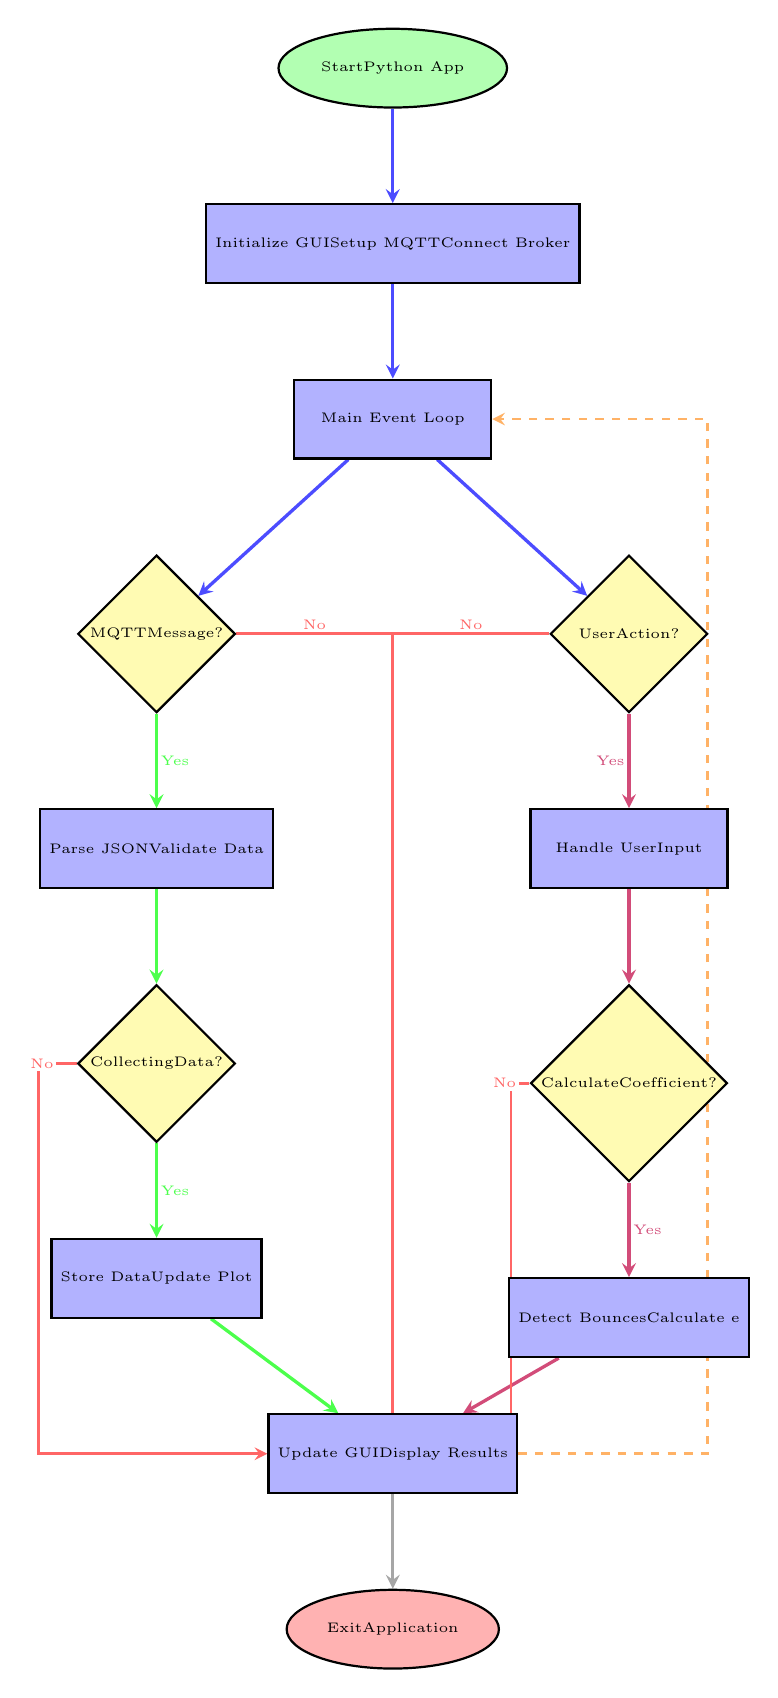
\begin{tikzpicture} [
    node distance=1.2cm,
    start/.style={ellipse, draw=black, thick, fill=green!30, minimum width=2.5cm, minimum height=1cm, font=\tiny, text centered},
    process/.style={rectangle, draw=black, thick, fill=blue!30, minimum width=2.5cm, minimum height=1cm, font=\tiny, text centered},
    decision/.style={diamond, draw=black, thick, fill=yellow!30, minimum width=2cm, minimum height=2cm, font=\tiny, text centered, inner sep=1pt},
    terminal/.style={ellipse, draw=black, thick, fill=red!30, minimum width=2cm, minimum height=1cm, font=\tiny, text centered},
    arrow/.style={->, thick, >=stealth}
]

% Layer 1: Define all nodes first (foreground)
\node[start] (start) {Start\\Python App};
\node[process, below=of start] (init) {Initialize GUI\\Setup MQTT\\Connect Broker};
\node[process, below=of init] (loop) {Main Event Loop};
\node[decision, below=of loop, xshift=-3cm] (mqtt_msg) {MQTT\\Message?};
\node[decision, below=of loop, xshift=3cm] (user_action) {User\\Action?};
\node[process, below=of mqtt_msg] (parse) {Parse JSON\\Validate Data};
\node[decision, below=of parse] (collecting) {Collecting\\Data?};
\node[process, below=of collecting] (store) {Store Data\\Update Plot};
\node[process, below=of user_action] (handle) {Handle User\\Input};
\node[decision, below=of handle] (analyze) {Calculate\\Coefficient?};
\node[process, below=of analyze] (calc) {Detect Bounces\\Calculate e};
\node[process, below=of store, xshift=3cm] (update) {Update GUI\\Display Results};
\node[terminal, below=of update] (end) {Exit\\Application};

% Layer 2: Draw all arrows in background
\begin{scope}[on background layer]
    % Main Flow Arrows
    \draw[arrow, blue!70, line width=1.2pt] (start) -- (init);
    \draw[arrow, blue!70, line width=1.2pt] (init) -- (loop);
    
    % Branch to decisions
    \draw[arrow, blue!70, line width=1.2pt] (loop) -- (mqtt_msg);
    \draw[arrow, blue!70, line width=1.2pt] (loop) -- (user_action);
    
    % MQTT Branch
    \draw[arrow, green!70, line width=1.2pt] (mqtt_msg) -- node[right, fill=white, inner sep=1pt, font=\tiny] {Yes} (parse);
    \draw[arrow, green!70, line width=1.2pt] (parse) -- (collecting);
    \draw[arrow, green!70, line width=1.2pt] (collecting) -- node[right, fill=white, inner sep=1pt, font=\tiny] {Yes} (store);
    \draw[arrow, green!70, line width=1.2pt] (store) -- (update);
    
    % User Branch
    \draw[arrow, purple!70, line width=1.2pt] (user_action) -- node[left, fill=white, inner sep=1pt, font=\tiny] {Yes} (handle);
    \draw[arrow, purple!70, line width=1.2pt] (handle) -- (analyze);
    \draw[arrow, purple!70, line width=1.2pt] (analyze) -- node[right, fill=white, inner sep=1pt, font=\tiny] {Yes} (calc);
    \draw[arrow, purple!70, line width=1.2pt] (calc) -- (update);
    
    % No Branches to Update
    \draw[arrow, red!60, line width=1pt] (mqtt_msg) -- node[above, fill=white, inner sep=1pt, font=\tiny] {No} ++(3,0) |- (update);
    \draw[arrow, red!60, line width=1pt] (user_action) -- node[above, fill=white, inner sep=1pt, font=\tiny] {No} ++(-3,0) |- (update);
    \draw[arrow, red!60, line width=1pt] (collecting) -- node[left, fill=white, inner sep=1pt, font=\tiny] {No} ++(-1.5,0) |- (update);
    \draw[arrow, red!60, line width=1pt] (analyze) -- node[left, fill=white, inner sep=1pt, font=\tiny] {No} ++(-1.5,0) |- (update);
    
    % Loop Back
    \draw[arrow, orange!60, line width=1pt, dashed] (update) -- ++(4,0) |- (loop);
    
    % Exit
    \draw[arrow, gray!70, line width=1.2pt] (update) -- (end);
\end{scope}

\end{tikzpicture}
\caption{Flowchart Program Python}
\end{figure}

\textbf{Penjelasan Program Python:} 

Aplikasi Python ini adalah program utama yang berfungsi sebagai pusat kontrol seluruh sistem monitoring koefisien restitusi bola. Program ini dirancang dengan antarmuka grafis (GUI) yang user-friendly menggunakan library Tkinter sehingga pengguna dapat dengan mudah mengoperasikan sistem tanpa perlu memahami kode programming.

\textbf{Cara Kerja Program Python:}
\begin{enumerate}
\item \textbf{Inisialisasi Sistem:} Saat program dimulai, sistem melakukan setup GUI (tampilan aplikasi), mengatur koneksi MQTT ke cloud broker HiveMQ, dan mempersiapkan semua komponen yang diperlukan untuk monitoring real-time.

\item \textbf{Loop Utama Monitoring:} Program masuk ke dalam loop pemantauan kontinyu yang secara bersamaan memantau dua hal: (a) pesan data sensor yang dikirim ESP8266 melalui internet via MQTT, dan (b) interaksi pengguna seperti klik tombol atau pengaturan parameter.

\item \textbf{Penerimaan Data Sensor:} Ketika ESP8266 mengirim data jarak dalam format JSON melalui internet, program Python menerima, memvalidasi, dan mengonversi data jarak menjadi tinggi bola dengan rumus: tinggi\_bola = tinggi\_sensor - jarak\_terukur.

\item \textbf{Penyimpanan dan Visualisasi:} Data yang valid disimpan dalam array waktu dan tinggi, kemudian divisualisasikan secara real-time dalam grafik yang terus ter-update untuk memudahkan observasi pergerakan bola.

\item \textbf{Analisis Otomatis:} Sistem menggunakan algoritma deteksi puncak untuk mengidentifikasi titik-titik pantulan bola, menghitung koefisien restitusi dengan rumus fisika $e = \sqrt{h_2/h_1}$, dan menghasilkan laporan komprehensif tentang karakteristik elastisitas bola.
\end{enumerate}

\newpage

\subsection{Flowchart Program ESP8266}

\begin{figure}[H]
\centering
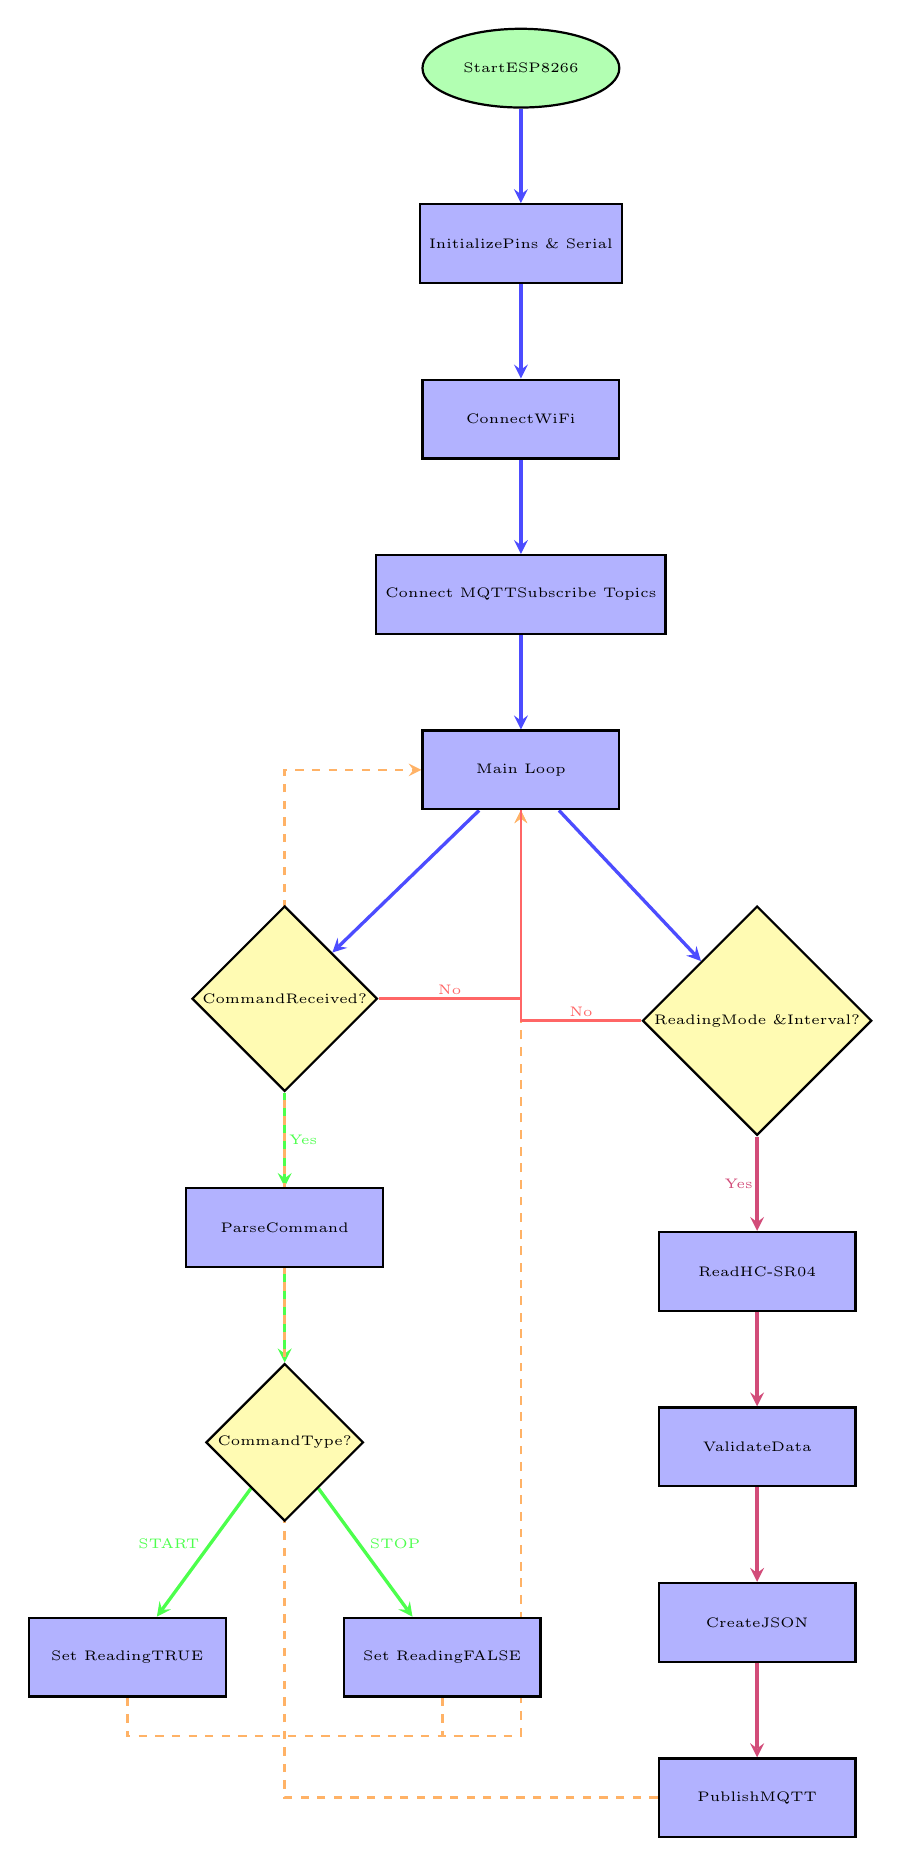
\begin{tikzpicture} [
    node distance=1.2cm,
    start/.style={ellipse, draw=black, thick, fill=green!30, minimum width=2.5cm, minimum height=1cm, font=\tiny, text centered},
    process/.style={rectangle, draw=black, thick, fill=blue!30, minimum width=2.5cm, minimum height=1cm, font=\tiny, text centered},
    decision/.style={diamond, draw=black, thick, fill=yellow!30, minimum width=2cm, minimum height=2cm, font=\tiny, text centered, inner sep=1pt},
    arrow/.style={->, thick, >=stealth}
]

% Layer 1: Define all nodes first (foreground)
\node[start] (start) {Start\\ESP8266};
\node[process, below=of start] (init_hw) {Initialize\\Pins \& Serial};
\node[process, below=of init_hw] (wifi) {Connect\\WiFi};
\node[process, below=of wifi] (mqtt) {Connect MQTT\\Subscribe Topics};
\node[process, below=of mqtt] (main_loop) {Main Loop};
\node[decision, below=of main_loop, xshift=-3cm] (cmd_check) {Command\\Received?};
\node[decision, below=of main_loop, xshift=3cm] (read_check) {Reading\\Mode \&\\Interval?};
\node[process, below=of cmd_check] (parse_cmd) {Parse\\Command};
\node[decision, below=of parse_cmd] (cmd_type) {Command\\Type?};
\node[process, below=of cmd_type, xshift=-2cm] (start_read) {Set Reading\\TRUE};
\node[process, below=of cmd_type, xshift=2cm] (stop_read) {Set Reading\\FALSE};
\node[process, below=of read_check] (sensor) {Read\\HC-SR04};
\node[process, below=of sensor] (validate) {Validate\\Data};
\node[process, below=of validate] (json) {Create\\JSON};
\node[process, below=of json] (publish) {Publish\\MQTT};

% Layer 2: Draw all arrows in background
\begin{scope}[on background layer]
    % Main Flow
    \draw[arrow, blue!70, line width=1.2pt] (start) -- (init_hw);
    \draw[arrow, blue!70, line width=1.2pt] (init_hw) -- (wifi);
    \draw[arrow, blue!70, line width=1.2pt] (wifi) -- (mqtt);
    \draw[arrow, blue!70, line width=1.2pt] (mqtt) -- (main_loop);
    
    % Branches
    \draw[arrow, blue!70, line width=1.2pt] (main_loop) -- (cmd_check);
    \draw[arrow, blue!70, line width=1.2pt] (main_loop) -- (read_check);
    
    % Command Flow
    \draw[arrow, green!70, line width=1.2pt] (cmd_check) -- node[right, fill=white, inner sep=1pt, font=\tiny] {Yes} (parse_cmd);
    \draw[arrow, green!70, line width=1.2pt] (parse_cmd) -- (cmd_type);
    \draw[arrow, green!70, line width=1.2pt] (cmd_type) -- node[above left, fill=white, inner sep=1pt, font=\tiny] {START} (start_read);
    \draw[arrow, green!70, line width=1.2pt] (cmd_type) -- node[above right, fill=white, inner sep=1pt, font=\tiny] {STOP} (stop_read);
    
    % Sensor Flow
    \draw[arrow, purple!70, line width=1.2pt] (read_check) -- node[left, fill=white, inner sep=1pt, font=\tiny] {Yes} (sensor);
    \draw[arrow, purple!70, line width=1.2pt] (sensor) -- (validate);
    \draw[arrow, purple!70, line width=1.2pt] (validate) -- (json);
    \draw[arrow, purple!70, line width=1.2pt] (json) -- (publish);
    
    % Loop Back
    \draw[arrow, orange!60, line width=1pt, dashed] (start_read) |- ++(0,-1) -| (main_loop);
    \draw[arrow, orange!60, line width=1pt, dashed] (stop_read) |- ++(0,-1) -| (main_loop);
    \draw[arrow, orange!60, line width=1pt, dashed] (publish) |- ++(-6,0) |- (main_loop);
    
    % No Action
    \draw[arrow, red!60, line width=1pt] (cmd_check) -- node[above, fill=white, inner sep=1pt, font=\tiny] {No} ++(3,0) |- (main_loop);
    \draw[arrow, red!60, line width=1pt] (read_check) -- node[above, fill=white, inner sep=1pt, font=\tiny] {No} ++(-3,0) |- (main_loop);
\end{scope}

\end{tikzpicture}
\caption{Flowchart Program ESP8266}
\end{figure}

\textbf{Penjelasan Program ESP8266:}

Program ESP8266 berperan sebagai sensor node cerdas yang bekerja secara autonomous (mandiri) untuk mengukur jarak menggunakan sensor ultrasonik HC-SR04 dan mengirimkan data ke aplikasi Python melalui komunikasi internet menggunakan protokol MQTT.

\textbf{Cara Kerja Program ESP8266:}
\begin{enumerate}
\item \textbf{Inisialisasi Hardware:} Saat ESP8266 dinyalakan, program melakukan setup pin GPIO untuk sensor HC-SR04 (pin trigger dan echo), mengatur komunikasi serial untuk debugging, dan menginisialisasi LED built-in sebagai indikator status.

\item \textbf{Koneksi WiFi:} ESP8266 terhubung ke jaringan WiFi menggunakan SSID dan password yang telah dikonfigurasi, memungkinkan akses internet untuk komunikasi dengan broker MQTT cloud.

\item \textbf{Setup MQTT:} Setelah WiFi terhubung, ESP8266 melakukan koneksi ke broker MQTT di cloud (HiveMQ), subscribe ke topik command untuk menerima perintah dari Python, dan siap mempublikasikan data sensor.

\item \textbf{Loop Pemrosesan Command:} Dalam loop utama, ESP8266 memantau perintah dari aplikasi Python seperti START\_READING (mulai pembacaan kontinyu), STOP\_READING (hentikan pembacaan), atau INTERVAL:nilai (ubah frekuensi pembacaan).

\item \textbf{Pembacaan Sensor:} Ketika mode pembacaan aktif, ESP8266 melakukan pengukuran jarak menggunakan HC-SR04 dengan mengirim gelombang ultrasonik dan menghitung waktu tempuh, kemudian mengkonversi ke jarak dalam satuan centimeter.

\item \textbf{Validasi dan Pengiriman Data:} Setiap hasil pembacaan divalidasi (rentang 2-400cm), dikemas dalam format JSON dengan timestamp yang direset setiap START\_READING, dan dikirim ke aplikasi Python melalui topik MQTT.
\end{enumerate}

\newpage

\subsection{Diagram Komunikasi Sistem}

\begin{figure}[H]
\centering
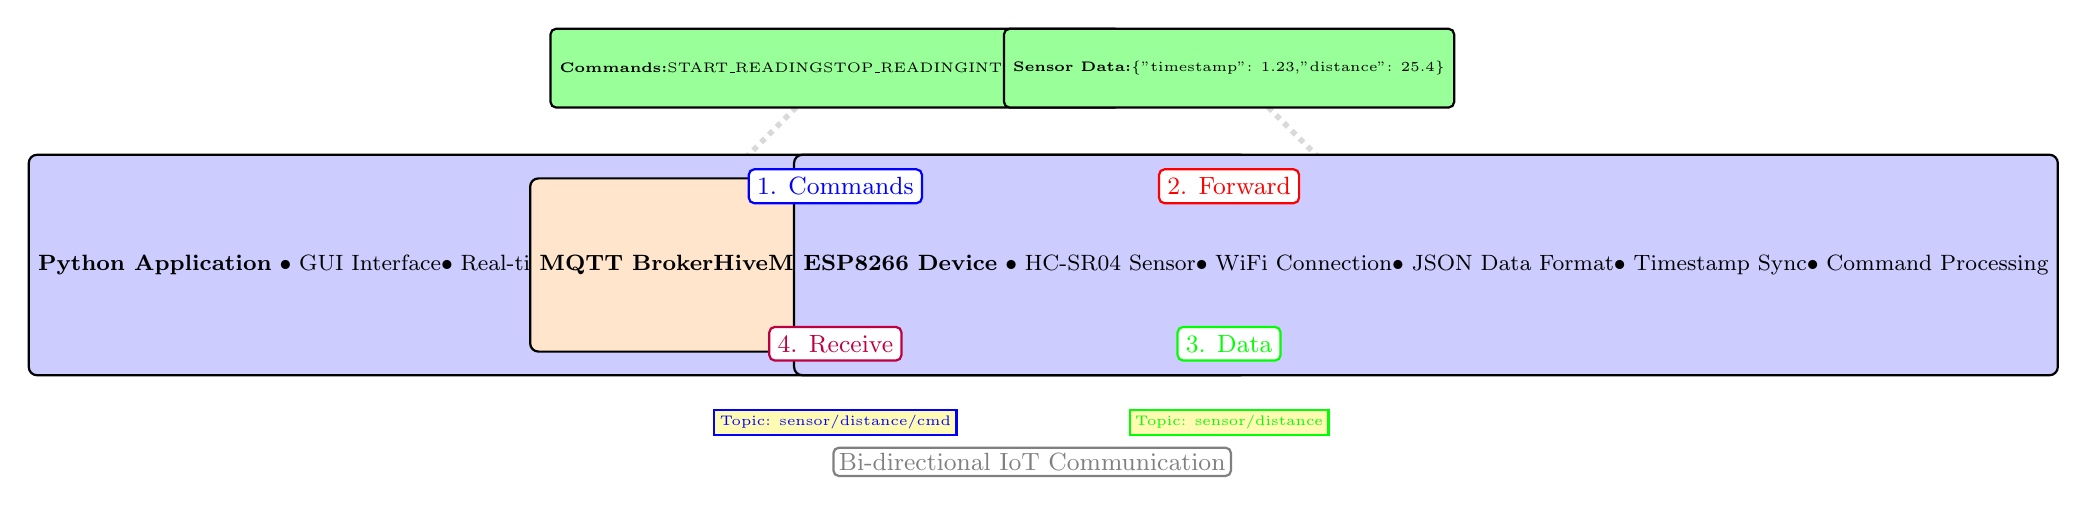
\begin{tikzpicture} [
    node distance=4cm,
    component/.style={rectangle, draw=black, thick, fill=blue!20, minimum width=3.5cm, minimum height=2.8cm, font=\footnotesize, text centered, rounded corners=3pt},
    broker/.style={rectangle, draw=black, thick, fill=orange!20, minimum width=3cm, minimum height=2.2cm, font=\footnotesize, text centered, rounded corners=3pt},
    data/.style={rectangle, draw=black, thick, fill=green!20, minimum width=3cm, minimum height=1cm, font=\tiny, text centered, rounded corners=2pt},
    arrow/.style={->, thick, >=stealth}
]

% LAYER 1: Draw background connections first
\draw[arrow, blue!40, line width=3pt] (0,0) -- (5,0);
\draw[arrow, red!40, line width=3pt] (5,0) -- (10,0);  
\draw[arrow, green!40, line width=3pt] (10,0) -- (5,0);
\draw[arrow, purple!40, line width=3pt] (5,0) -- (0,0);

\draw[dotted, gray!30, line width=2pt] (2.5,2.5) -- (0,0);
\draw[dotted, gray!30, line width=2pt] (7.5,2.5) -- (10,0);

\draw[arrow, dashed, gray!20, line width=4pt] (0,0) -- (10,0);

% LAYER 2: Draw nodes on top
\node[component] (python) at (0,0) {
    \textbf{Python Application}\\[0.2cm]
    $\bullet$ GUI Interface\\
    $\bullet$ Real-time Monitoring\\
    $\bullet$ Data Analysis\\
    $\bullet$ Coefficient Calculation\\
    $\bullet$ File Export
};

\node[broker] (mqtt_broker) at (5,0) {
    \textbf{MQTT Broker}\\
    \textbf{HiveMQ Cloud}\\[0.1cm]
    $\bullet$ Message Routing\\
    $\bullet$ Real-time Delivery\\
    $\bullet$ Topic Management
};

\node[component] (esp8266) at (10,0) {
    \textbf{ESP8266 Device}\\[0.2cm]
    $\bullet$ HC-SR04 Sensor\\
    $\bullet$ WiFi Connection\\
    $\bullet$ JSON Data Format\\
    $\bullet$ Timestamp Sync\\
    $\bullet$ Command Processing
};

\node[data, fill=green!40] (cmd_data) at (2.5,2.5) {
    \textbf{Commands:}\\
    START\_READING\\
    STOP\_READING\\
    INTERVAL:value
};

\node[data, fill=green!40] (sensor_data) at (7.5,2.5) {
    \textbf{Sensor Data:}\\
    \{"timestamp": 1.23,\\
    "distance": 25.4\}
};

% LAYER 3: Add labels on top of everything
\node[font=\small, text=blue, fill=white, inner sep=3pt, draw=blue, thick, rounded corners=2pt] at (2.5,1) {1. Commands};
\node[font=\small, text=red, fill=white, inner sep=3pt, draw=red, thick, rounded corners=2pt] at (7.5,1) {2. Forward};
\node[font=\small, text=green, fill=white, inner sep=3pt, draw=green, thick, rounded corners=2pt] at (7.5,-1) {3. Data};
\node[font=\small, text=purple, fill=white, inner sep=3pt, draw=purple, thick, rounded corners=2pt] at (2.5,-1) {4. Receive};

\node[font=\tiny, text=blue, fill=yellow!30, inner sep=2pt, draw=blue, thick] at (2.5,-2) {Topic: sensor/distance/cmd};
\node[font=\tiny, text=green, fill=yellow!30, inner sep=2pt, draw=green, thick] at (7.5,-2) {Topic: sensor/distance};

\node[font=\small, text=gray, fill=white, inner sep=2pt, draw=gray, thick, rounded corners=2pt] at (5,-2.5) {Bi-directional IoT Communication};

\end{tikzpicture}
\caption{Arsitektur Komunikasi MQTT Sistem IoT}
\end{figure}

\textbf{Komunikasi Sistem IoT:}

Sistem ini mengimplementasikan arsitektur Internet of Things (IoT) modern berbasis protokol MQTT yang memungkinkan komunikasi real-time antara perangkat sensor (ESP8266) dan aplikasi monitoring (Python) melalui internet menggunakan cloud broker HiveMQ yang tersedia 24/7.

\textbf{Penjelasan Detail Alur Komunikasi:}

\begin{enumerate}
\item \textbf{Pengiriman Command (Python → MQTT Broker):} Aplikasi Python mengirimkan perintah kontrol seperti "START\_READING" atau "STOP\_READING" ke broker MQTT cloud melalui topik khusus "sensor/distance/cmd". Perintah ini dikirim dalam format teks sederhana yang mudah dipahami ESP8266.

\item \textbf{Penerusan Command (MQTT Broker → ESP8266):} Broker MQTT cloud secara otomatis meneruskan semua perintah yang diterima dari Python ke ESP8266 yang telah subscribe ke topik command. Proses ini terjadi dalam hitungan milidetik berkat infrastruktur cloud yang cepat.

\item \textbf{Pengiriman Data Sensor (ESP8266 → MQTT Broker):} Setelah menerima perintah START\_READING, ESP8266 mulai mengukur jarak menggunakan sensor HC-SR04 secara kontinyu dan mengirimkan data dalam format JSON ke broker MQTT melalui topik "sensor/distance". Data JSON berisi timestamp, jarak terukur, dan identitas perangkat.

\item \textbf{Penerimaan Data (MQTT Broker → Python):} Aplikasi Python yang telah subscribe ke topik data sensor menerima semua data yang dikirim ESP8266 melalui broker. Data JSON ini kemudian di-parse, divalidasi, dan dikonversi menjadi informasi tinggi bola untuk analisis real-time.
\end{enumerate}

\textbf{Keunggulan Arsitektur MQTT:}
\begin{itemize}
\item \textbf{Komunikasi Real-time:} Latensi rendah untuk monitoring langsung pergerakan bola
\item \textbf{Reliability:} Broker cloud menjamin pengiriman pesan dengan mekanisme Quality of Service (QoS)
\item \textbf{Scalability:} Dapat dengan mudah menambahkan multiple ESP8266 atau aplikasi monitoring
\item \textbf{Internet-based:} Monitoring dapat dilakukan dari jarak jauh selama ada koneksi internet
\item \textbf{Bi-directional:} Komunikasi dua arah memungkinkan kontrol penuh terhadap sistem sensor
\end{itemize}

\subsection{Spesifikasi Teknis}

\subsubsection{Format Data JSON}
\begin{itemize}
    \item \textbf{Sensor Data:} \texttt{\{"timestamp": 1.23, "distance": 25.4, "device": "ESP8266\_HCSR04"\}}
    \item \textbf{Commands:} \texttt{START\_READING}, \texttt{STOP\_READING}, \texttt{INTERVAL:100}
\end{itemize}

\subsubsection{Parameter Sistem}
\begin{itemize}
    \item \textbf{Sensor Range:} 2-400 cm
    \item \textbf{Sampling Rate:} 50-5000 ms (configurable)
    \item \textbf{Analysis Formula:} $e = \sqrt{\frac{h_2}{h_1}}$
    \item \textbf{MQTT Topics:} sensor/distance, sensor/distance/cmd
\end{itemize}

\subsection{Diagram Alir untuk melakukan percobaan}

\begin{figure}[H]
\centering
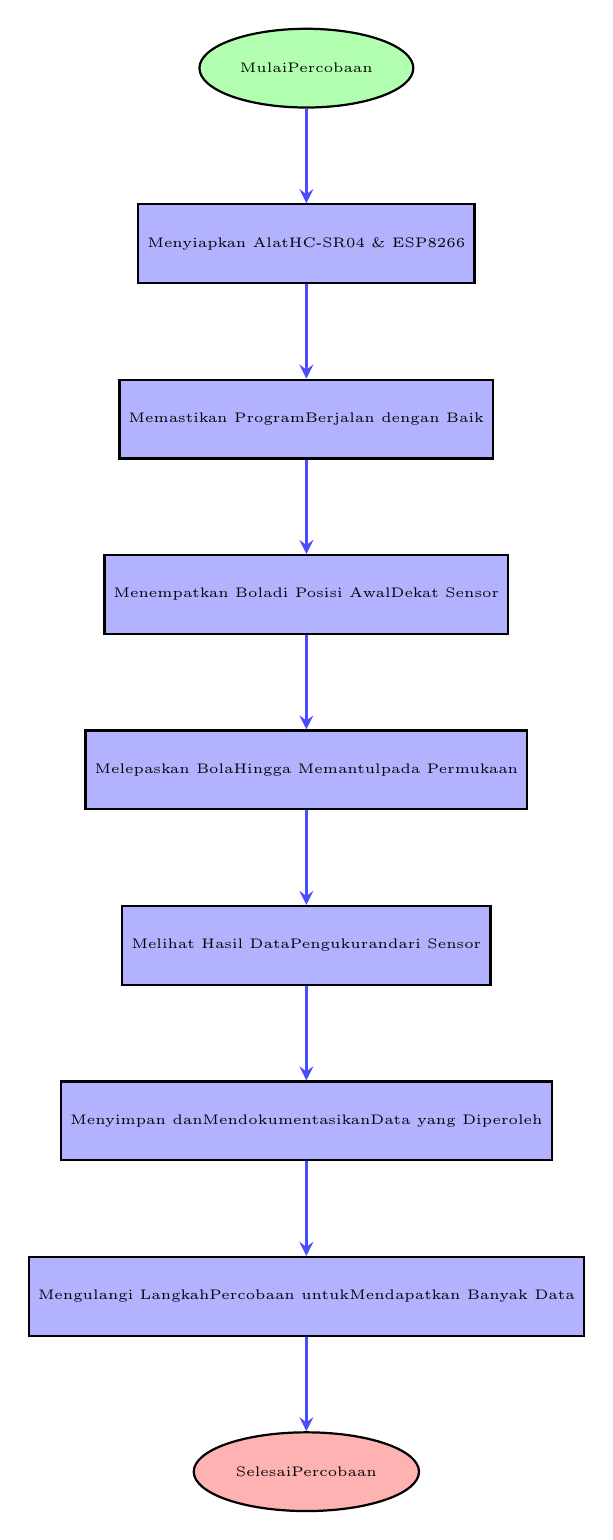
\begin{tikzpicture} [
    node distance=1.2cm,
    start/.style={ellipse, draw=black, thick, fill=green!30, minimum width=2.5cm, minimum height=1cm, font=\tiny, text centered},
    process/.style={rectangle, draw=black, thick, fill=blue!30, minimum width=2.5cm, minimum height=1cm, font=\tiny, text centered},
    terminal/.style={ellipse, draw=black, thick, fill=red!30, minimum width=2cm, minimum height=1cm, font=\tiny, text centered},
    arrow/.style={->, thick, >=stealth}
]

% Define all nodes first (foreground)
\node[start] (start) {Mulai\\Percobaan};
\node[process, below=of start] (alat) {Menyiapkan Alat\\HC-SR04 \& ESP8266};
\node[process, below=of alat] (program) {Memastikan Program\\Berjalan dengan Baik};
\node[process, below=of program] (posisi) {Menempatkan Bola\\di Posisi Awal\\Dekat Sensor};
\node[process, below=of posisi] (lepas) {Melepaskan Bola\\Hingga Memantul\\pada Permukaan};
\node[process, below=of lepas] (lihat) {Melihat Hasil Data\\Pengukuran\\dari Sensor};
\node[process, below=of lihat] (simpan) {Menyimpan dan\\Mendokumentasikan\\Data yang Diperoleh};
\node[process, below=of simpan] (ulang) {Mengulangi Langkah\\Percobaan untuk\\Mendapatkan Banyak Data};
\node[terminal, below=of ulang] (end) {Selesai\\Percobaan};

% Draw all arrows in background
\begin{scope}[on background layer]
    \draw[arrow, blue!70, line width=1.2pt] (start) -- (alat);
    \draw[arrow, blue!70, line width=1.2pt] (alat) -- (program);
    \draw[arrow, blue!70, line width=1.2pt] (program) -- (posisi);
    \draw[arrow, blue!70, line width=1.2pt] (posisi) -- (lepas);
    \draw[arrow, blue!70, line width=1.2pt] (lepas) -- (lihat);
    \draw[arrow, blue!70, line width=1.2pt] (lihat) -- (simpan);
    \draw[arrow, blue!70, line width=1.2pt] (simpan) -- (ulang);
    \draw[arrow, blue!70, line width=1.2pt] (ulang) -- (end);
\end{scope}

\end{tikzpicture}
\caption{Flowchart Prosedur Percobaan}
\end{figure}

\textbf{Penjelasan Prosedur Percobaan:}

Flowchart prosedur percobaan ini menggambarkan metodologi sistematis untuk melakukan pengukuran koefisien restitusi bola menggunakan teknologi IoT modern. Setiap langkah dirancang untuk memastikan akurasi data dan reproducibility hasil eksperimen.

\textbf{Cara Kerja Prosedur Percobaan:}
\begin{enumerate}
\item \textbf{Persiapan Perangkat Keras:} Tahap awal meliputi setup fisik sistem IoT dengan menempatkan sensor HC-SR04 pada ketinggian terukur dari lantai, menghubungkan ESP8266 ke power supply, dan memastikan semua koneksi hardware (trigger pin, echo pin, WiFi antenna) berfungsi optimal. Kalibrasi sensor dilakukan untuk memastikan pembacaan jarak yang akurat dalam rentang 2-400cm.

\item \textbf{Validasi Sistem Software:} Sebelum eksperimen dimulai, dilakukan pengecekan menyeluruh terhadap koneksi WiFi ESP8266, status MQTT broker connection ke HiveMQ Cloud, dan responsivitas komunikasi antara aplikasi Python dengan device sensor. Test komunikasi dilakukan dengan mengirim command sederhana dan memverifikasi response time.

\item \textbf{Setup Eksperimental:} Bola ditempatkan pada posisi awal yang tepat di bawah sensor HC-SR04 dengan jarak optimal (biasanya 10-30cm dari sensor) untuk memastikan deteksi yang akurat. Lingkungan eksperimen harus bebas dari interferensi suara dan getaran yang dapat mempengaruhi sensor ultrasonik.

\item \textbf{Eksekusi Pengukuran:} Saat bola dilepaskan, sistem mulai melakukan continuous monitoring dengan sampling rate tinggi (50-100ms interval). Data jarak real-time dikirim via MQTT dalam format JSON yang berisi timestamp presisi tinggi, nilai jarak, dan metadata perangkat untuk tracking yang akurat.

\item \textbf{Real-time Data Monitoring:} Operator memantau grafik real-time di aplikasi Python untuk memastikan kualitas data yang dikumpulkan. Visual feedback memungkinkan deteksi immediate terhadap anomali atau error dalam pengukuran, seperti noise berlebihan atau pembacaan yang tidak konsisten.

\item \textbf{Data Persistence dan Backup:} Setiap sesi pengukuran secara otomatis disimpan dalam multiple format (Excel untuk analisis statistik, JSON untuk processing lebih lanjut, dan PNG untuk dokumentasi visual). Timestamping dan naming convention yang konsisten memudahkan organization dan retrieval data.

\item \textbf{Replicability dan Statistical Validity:} Proses diulang multiple kali (minimum 5-10 repetisi) untuk memperoleh dataset yang statistik significant. Variasi antar-percobaan dianalisis untuk memastikan consistency dan mengidentifikasi potential systematic errors.

\item \textbf{Quality Control dan Documentation:} Setiap sesi percobaan didokumentasikan dengan metadata lengkap termasuk environmental conditions, ball specifications, sensor configuration, dan observation notes untuk memastikan traceability dan reproducibility eksperimen.
\end{enumerate}

\newpage

\subsection{Diagram Alir untuk mengolah data}

\begin{figure}[H]
\centering
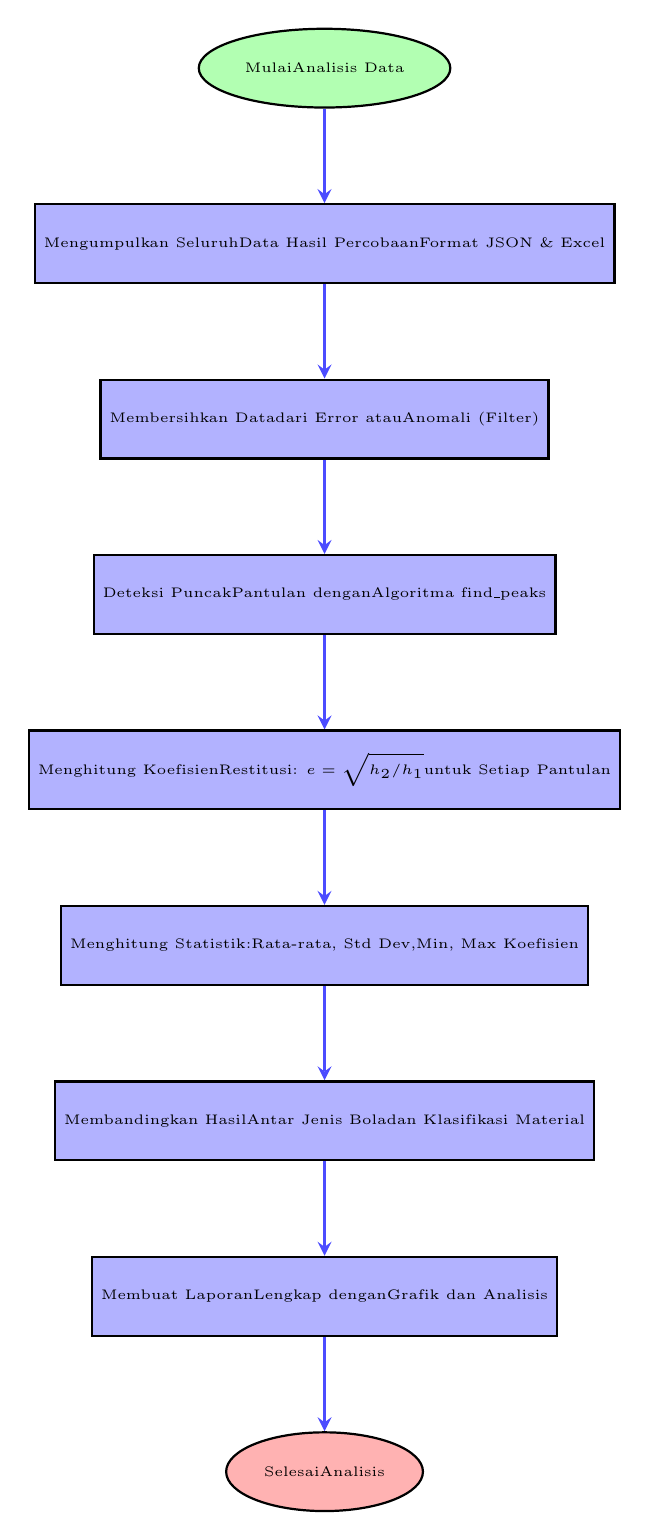
\begin{tikzpicture} [
    node distance=1.2cm,
    start/.style={ellipse, draw=black, thick, fill=green!30, minimum width=2.5cm, minimum height=1cm, font=\tiny, text centered},
    process/.style={rectangle, draw=black, thick, fill=blue!30, minimum width=2.5cm, minimum height=1cm, font=\tiny, text centered},
    terminal/.style={ellipse, draw=black, thick, fill=red!30, minimum width=2cm, minimum height=1cm, font=\tiny, text centered},
    arrow/.style={->, thick, >=stealth}
]

% Define all nodes first (foreground)
\node[start] (start) {Mulai\\Analisis Data};
\node[process, below=of start] (kumpul) {Mengumpulkan Seluruh\\Data Hasil Percobaan\\Format JSON \& Excel};
\node[process, below=of kumpul] (bersih) {Membersihkan Data\\dari Error atau\\Anomali (Filter)};
\node[process, below=of bersih] (deteksi) {Deteksi Puncak\\Pantulan dengan\\Algoritma find\_peaks};
\node[process, below=of deteksi] (hitung) {Menghitung Koefisien\\Restitusi: $e = \sqrt{h_2/h_1}$\\untuk Setiap Pantulan};
\node[process, below=of hitung] (statistik) {Menghitung Statistik:\\Rata-rata, Std Dev,\\Min, Max Koefisien};
\node[process, below=of statistik] (banding) {Membandingkan Hasil\\Antar Jenis Bola\\dan Klasifikasi Material};
\node[process, below=of banding] (laporan) {Membuat Laporan\\Lengkap dengan\\Grafik dan Analisis};
\node[terminal, below=of laporan] (end) {Selesai\\Analisis};

% Draw all arrows in background
\begin{scope}[on background layer]
    \draw[arrow, blue!70, line width=1.2pt] (start) -- (kumpul);
    \draw[arrow, blue!70, line width=1.2pt] (kumpul) -- (bersih);
    \draw[arrow, blue!70, line width=1.2pt] (bersih) -- (deteksi);
    \draw[arrow, blue!70, line width=1.2pt] (deteksi) -- (hitung);
    \draw[arrow, blue!70, line width=1.2pt] (hitung) -- (statistik);
    \draw[arrow, blue!70, line width=1.2pt] (statistik) -- (banding);
    \draw[arrow, blue!70, line width=1.2pt] (banding) -- (laporan);
    \draw[arrow, blue!70, line width=1.2pt] (laporan) -- (end);
\end{scope}

\end{tikzpicture}
\caption{Flowchart Analisis dan Pengolahan Data}
\end{figure}

\textbf{Penjelasan Proses Pengolahan Data:}

Flowchart pengolahan data menunjukkan pipeline analisis yang sophisticated untuk mengekstrak koefisien restitusi dari raw sensor data. Setiap tahap menggunakan algoritma advanced untuk memastikan akurasi dan validitas hasil analisis.

\textbf{Cara Kerja Pengolahan Data:}
\begin{enumerate}
\item \textbf{Data Aggregation dan Import:} Sistem mengumpulkan semua file data dari multiple experiment sessions, melakukan parsing format JSON dan Excel, dan memvalidasi data integrity. Error checking dilakukan untuk mendeteksi corrupted files, missing timestamps, atau inconsistent data ranges yang dapat mempengaruhi analisis.

\item \textbf{Data Preprocessing dan Noise Reduction:} Raw sensor data dibersihkan menggunakan sophisticated filtering techniques termasuk low-pass Butterworth filter untuk menghilangkan high-frequency noise, outlier detection menggunakan statistical methods (IQR dan Z-score), dan data interpolation untuk mengisi missing data points yang minimal.

\item \textbf{Peak Detection Algorithm:} Implementasi algoritma `find_peaks` dari SciPy dengan parameter optimization untuk mendeteksi bounce peaks yang akurat. Algorithm menggunakan multiple criteria termasuk minimum height threshold, prominence analysis, dan distance constraints untuk mengidentifikasi true bounce events sambil mengeliminasi false positives.

\item \textbf{Physics-based Coefficient Calculation:} Untuk setiap pasangan consecutive bounces, sistem menghitung koefisien restitusi menggunakan rumus fundamental fisika $e = \sqrt{h_2/h_1}$ dimana $h_1$ adalah tinggi bounce pertama dan $h_2$ adalah tinggi bounce kedua. Validasi dilakukan untuk memastikan $0 < e < 1$ sesuai dengan physical constraints.

\item \textbf{Statistical Analysis dan Uncertainty Quantification:} Comprehensive statistical analysis dilakukan termasuk calculation of mean, standard deviation, confidence intervals, dan distribution analysis. Uncertainty propagation dihitung untuk memahami error margins dan reliability dari hasil pengukuran.

\item \textbf{Comparative Analysis dan Material Classification:} Results dibandingkan dengan theoretical values dan empirical data dari literature untuk material classification. Machine learning algorithms dapat diimplementasikan untuk automated material identification berdasarkan bounce characteristics dan coefficient patterns.

\item \textbf{Report Generation dan Visualization:} Sistem menghasilkan comprehensive reports dengan high-quality visualizations termasuk time-series plots, bounce trajectory analysis, statistical distributions, dan comparison charts. Reports di-format dalam multiple outputs (PDF untuk presentation, Excel untuk further analysis, HTML untuk web sharing).

\item \textbf{Data Quality Assessment dan Validation:} Final stage meliputi comprehensive validation terhadap hasil analisis, consistency checking dengan physical laws, dan assessment terhadap experimental uncertainty. Quality metrics dihitung untuk mengevaluasi reliability dan accuracy dari entire measurement dan analysis process.
\end{enumerate}

\textbf{Advanced Features dalam Pengolahan Data:}

\begin{itemize}
\item \textbf{Automated Algorithm Optimization:} Sistem secara otomatis menyesuaikan parameter detection algorithm berdasarkan karakteristik specific dari setiap ball type dan experimental conditions.

\item \textbf{Multi-dimensional Analysis:} Selain koefisien restitusi, sistem juga menganalisis parameter tambahan seperti energy loss rate, bounce frequency, dan damping characteristics untuk comprehensive material characterization.

\item \textbf{Error Propagation Analysis:} Sophisticated uncertainty analysis yang memperhitungkan semua source of error mulai dari sensor accuracy, timing precision, environmental factors, hingga computational rounding errors.

\item \textbf{Real-time Feedback Loop:} Integration dengan experimental setup memungkinkan real-time adjustment terhadap measurement parameters berdasarkan preliminary analysis results untuk optimization data quality.

\item \textbf{Database Integration:} Results dapat disimpan dalam structured database format untuk long-term storage, easy retrieval, dan meta-analysis across multiple experiments dan ball types.
\end{itemize}

\end{document}